\documentclass[../tb_report.tex]{subfiles}

\begin{document}

\chapter{Proof of space}
\label{ch:pospace}

\section{Introduction}

La \emph{preuve d'espace} (ou \emph{proof of space} en anglais) est un algorithme de consensus similaire à la preuve de travail à la différence qu'au lieu d'effectuer des calculs de manière continue pour trouver une preuve satisfaisant les conditions de la difficulté de la blockchain, les mineurs appelés farmers avec \emph{PoSpace} vont trouver des preuves à partir d'un challenge grâce à une certaine quantité de données allouées sur le disque dur. Ces données sont générées préalablement par le farmer dans une étape appelée \textbf{plotting}. Ce sont des données pseudo-aléatoires qui ne représentent rien de particulier. D'autres algorithmes pour stocker des données utiles existent comme \emph{proof of catalytic space} ou \emph{proof of replication}.

En suite, un farmer peut prouver qu'il a bien les données qu'il dit avoir stockées en trouvant une ou plusieurs preuves répondant à un challenge donné. C'est l'étape du \textbf{farming}.

Lors de la \textbf{vérification}, le vérificateur récupère la prevue est à partir de celle-ci, recalcule le challenge et vérifie s'il correspond à celui envoyé précédemment.

Ainsi, on peut considérer \emph{proof of space} comme est un protocole dans lequel nous avons :

\begin{enumerate}
  \item un vérificateur qui envoie un challenge à un farmer et
  \item un farmer qui peut prouver au vérificateur qu'il a bien alloué la quantité d'espace spécifiée à un instant $t$.
\end{enumerate}

\begin{figure}[H]
  \centering
  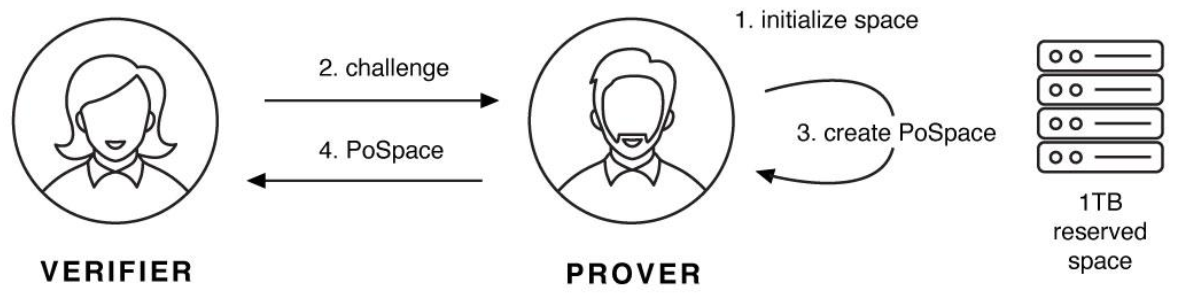
\includegraphics[width=\textwidth]{images/pospace.png}
  \caption{Diagramme du protocole \emph{proof of space} montrant les différentes étapes. Tiré de \cite{chia:consensus}}
\end{figure}

\section{Plotting}

Le plotting est un procédé non-interactif dans le lequel le farmer va créer les données qui seront stockées et qui permettront de trouver les preuves d'espace liées aux challenges. Ce procédé peut être long, cela peut prendre de plusieurs heures à plusieurs jours suivant la quantité de données allouées.

Le farmer choisi un nombre $k$ qui sera proportionnel à la quantité de données souhaitées. Le processus générera un plot dont la taille sera environ égale à $780 \times k \times 2^{k-10}$ \cite{chia:consensus}. Le temps de la génération dépend de la puissance de l'ordinateur effectuant le plotting comme il s'agit principalement d'exécution de fonctions de hachage, c'est le CPU qui sera beaucoup solicité durant cette étape. Le contenu du plot sera 4 tables de données pseudo-aléatoires. Chaque table contiendra $2^k$ entrées et chaque entrée d'une table $i$ pointra vers 2 entrées dans la table précédente ($i-1$). La première table quant à elle contientra ce qu'on appelle les \emph{x-values}. Ce sont simplement des nombres entiers de $0$ à $2^k-1$. Ainsi. une preuve d'espace correspond à 8 \emph{x-values} ($2^{\textsf{nombre de table} - 1} = 2^3 = 8$).

La construction de cette preuve d'espace est basée sur la construction de Chia \cite{chia:construction}, elle-même basée sur \emph{Beyond Hellman} \cite{DBLP:conf/asiacrypt/AbusalahACKPR17}. Elle a cependant été simplifiée pour pouvoir être réalisée dans le temps imparti de ce travail.

\section{Farming}

\dots

\section{Vérification}

\dots

\section{Sécurité et attaques}

\dots

\end{document}